% Created 2024-05-11 Sat 16:33
% Intended LaTeX compiler: xelatex
\documentclass[11pt]{article}
\usepackage{hyperref}
% TIPS
% \substack{a\\b} for multiple lines text





% pdfplots will load xolor automatically without option
\usepackage[dvipsnames]{xcolor}

\usepackage{forest}
% two-line text in node by [two \\ lines]
% \begin{forest} qtree, [..] \end{forest}
\forestset{
  qtree/.style={
    baseline,
    for tree={
      parent anchor=south,
      child anchor=north,
      align=center,
      inner sep=1pt,
    }}}
%\usepackage{flexisym}
% load order of mathtools and mathabx, otherwise conflict overbrace

\usepackage{mathtools}
%\usepackage{fourier}
\usepackage{pgfplots}
\usepackage{amsthm, mathabx,  amsmath, commath}
\usepackage{amsfonts}

\usepackage{empheq}
\usepackage{tikz}
\usetikzlibrary{arrows.meta}
\usepackage[most]{tcolorbox}

\newtheorem{theorem}{Theorem}[section]
\newtheorem{definition}{Definition}[section]
\newtheorem{corollary}{Corollary}[section]
\newtheorem{example}{Example}[section]
\newtheorem{lemma}{Lemma}[section]
\newtheorem{proposition}{Proposition}[section]

\newcommand{\bl}[1] {\boldsymbol{#1}}
\newcommand{\Wt}[1] {\stackrel{\sim}{\smash{#1}\rule{0pt}{1.1ex}}}
\newcommand{\wt}[1] {\widetilde{#1}}


%For boxed texts in align, use Aboxed{}
%otherwise use boxed{}

\DeclareMathSymbol{\widehatsym}{\mathord}{largesymbols}{"62}
\newcommand\lowerwidehatsym{%
  \text{\smash{\raisebox{-1.3ex}{%
    $\widehatsym$}}}}
\newcommand\fixwidehat[1]{%
  \mathchoice
    {\accentset{\displaystyle\lowerwidehatsym}{#1}}
    {\accentset{\textstyle\lowerwidehatsym}{#1}}
    {\accentset{\scriptstyle\lowerwidehatsym}{#1}}
    {\accentset{\scriptscriptstyle\lowerwidehatsym}{#1}}
}

\usepackage{graphicx}
    
% text on arrow for xRightarrow
\makeatletter
%\newcommand{\xRightarrow}[2][]{\ext@arrow 0359\Rightarrowfill@{#1}{#2}}
\makeatother


\def \bx {\boldsymbol{x}}
\def \ba {\boldsymbol{a}}
\def \bI {\boldsymbol{I}}
\def \bt {\boldsymbol{t}}
\def \bb {\boldsymbol{b}}
\def \bA {\boldsymbol{A}}
\def \bX {\boldsymbol{X}}
\def \bu {\boldsymbol{u}}
\def \bS {\boldsymbol{S}}
\def \bZ {\boldsymbol{Z}}
\def \bz {\boldsymbol{z}}
\def \by {\boldsymbol{y}}
\def \bw {\boldsymbol{w}}
\def \bT {\boldsymbol{T}}
\def \bS {\boldsymbol{S}}
\def \bm {\boldsymbol{m}}
\def \bW {\boldsymbol{W}}
\def \bY {\boldsymbol{Y}}
\def \bH {\boldsymbol{H}}
\def \blambda {\boldsymbol{\lambda}}
\def \bPhi {\boldsymbol{\Phi}}
\def \btheta {\boldsymbol{\theta}}
\def \bmu {\boldsymbol{\mu}}
\def \bphi {\boldsymbol{\phi}}
\def \bSigma {\boldsymbol{\Sigma}}
\def \lb {\left\{}
\def \rb {\right\}}
\def \caln {\mathcal{N}}
\def \dissum {\displaystyle\Sigma}
\def \dispro {\displaystyle\prod}
\def \E {\mathbb{E}}
\def \Q {\mathbb{Q}}
\def \V {\mathbb{V}}
\def \R {\mathbb{R}}
\def \calq {\mathcal{Q}}
\def \calg {\mathcal{G}}
\def \caln {\mathcal{N}}
\def \calr {\mathcal{R}}
\def \calm {\mathcal{M}}
\def \calc {\mathcal{C}}
\def \bcup {\bigcup}

\graphicspath{{../../../paper/consensus/}}

%% ox-latex features:
%   !announce-start, !guess-pollyglossia, !guess-babel, !guess-inputenc, caption,
%   underline, image, !announce-end.

\usepackage{capt-of}

\usepackage[normalem]{ulem}

\usepackage{graphicx}

%% end ox-latex features


\author{wu}
\date{\today}
\title{Consensus on Transaction Commit}
\hypersetup{
 pdfauthor={wu},
 pdftitle={Consensus on Transaction Commit},
 pdfkeywords={},
 pdfsubject={},
 pdfcreator={Emacs 29.1 (Org mode 9.7-pre)}, 
 pdflang={English}}
\begin{document}

\maketitle
\section{Transaction Commit}
\label{sec:orge8e52a5}
        We assume a set of RM processes, each beginning in a \textbf{working} state. The goal of the protocol is for
        the RMs all to reach a \textbf{committed} state or all to reach an \textbf{aborted} state.
Two safety requirements:
\begin{enumerate}
\item \textbf{Stability}: Once an RM has entered the \textbf{committed} or \textbf{aborted} state, it remains in that state forever.
\item \textbf{Consistency}: It is impossible for one RM to be in the \textbf{committed} state and another to be in the
\textbf{aborted} state.
\end{enumerate}

Each RM also has a \textbf{prepared} state. We require that
\begin{itemize}
\item An RM can enter the \textbf{committed} state only after all RMs have been in the \emph{prepared} state.
\end{itemize}

These requirements imply that the transaction can commit, meaning that all RMs reach the \textbf{committed}
state, only by the following sequence of events:
\begin{itemize}
\item All the RMs enter the \textbf{prepared} state, in any order
\item All the RMs enter the \textbf{committed} state, in any order
\end{itemize}

The protocol allows the following event that prevents the transaction from committing:
\begin{itemize}
\item Any RM in the \textbf{working} state can enter the \textbf{aborted} state.
\end{itemize}

\begin{center}
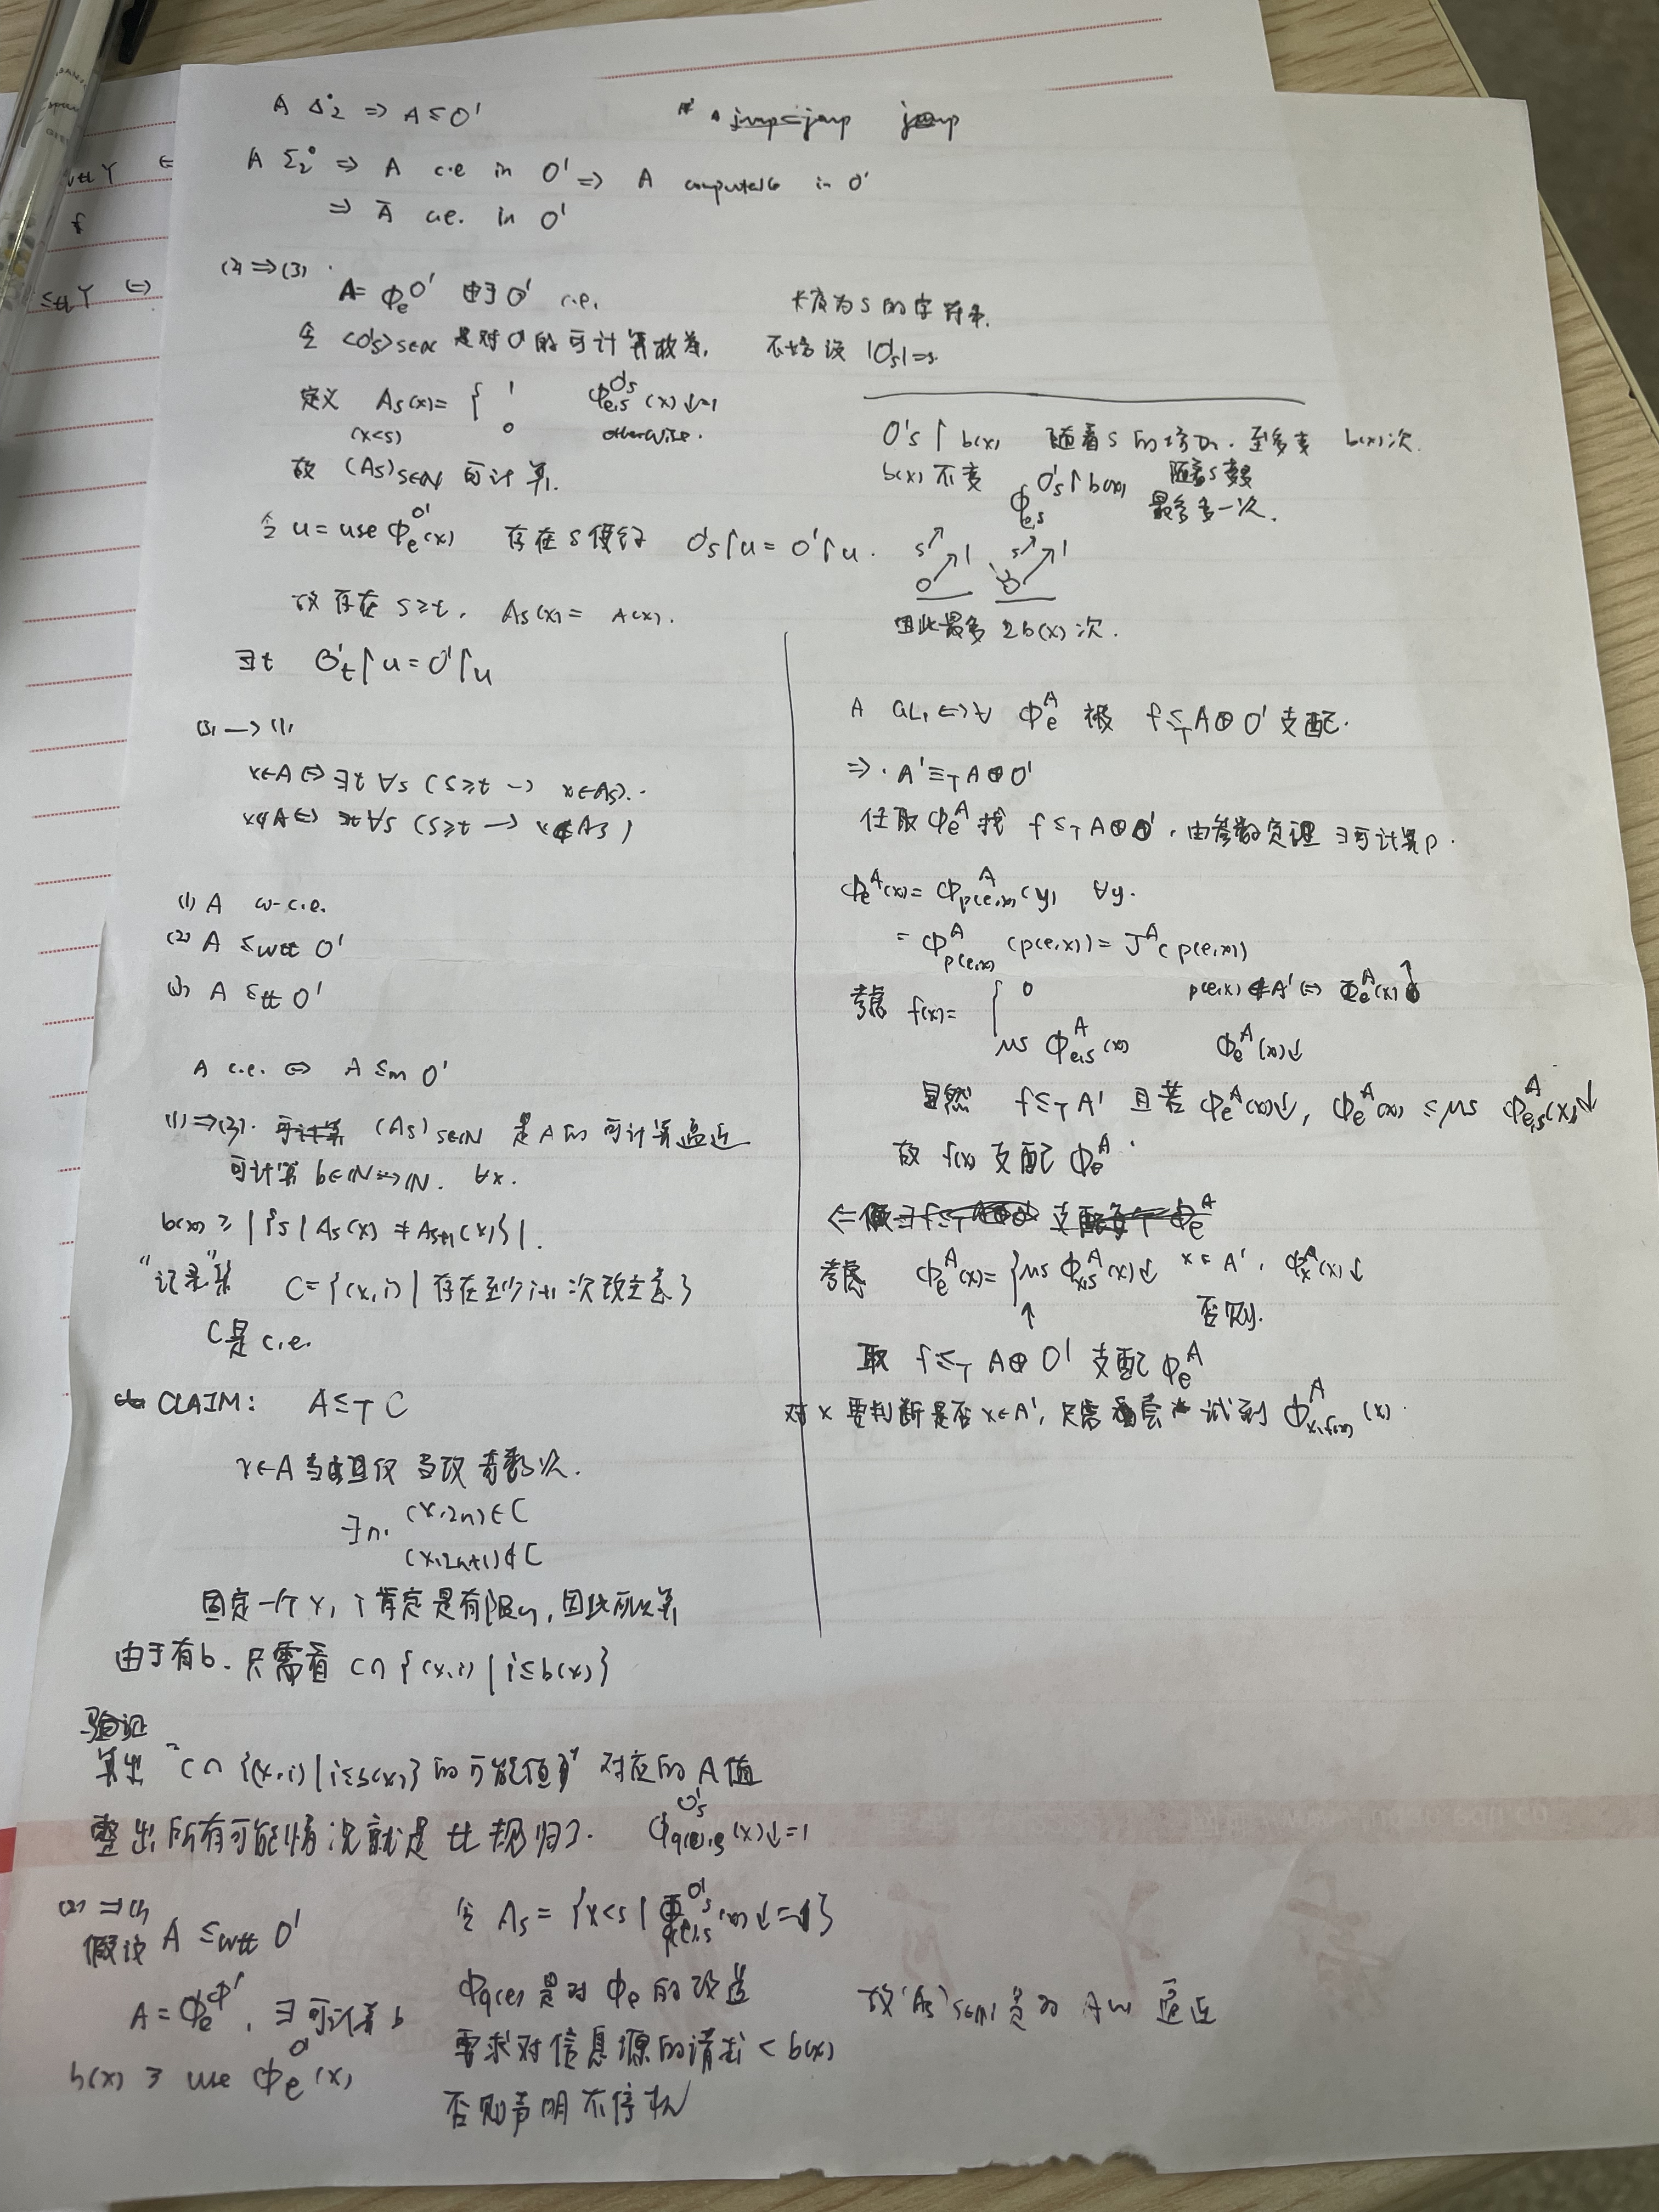
\includegraphics[width=.8\textwidth]{../../images/papers/1.png}
\label{}
\end{center}

The goal of the algorithm is for all RMs to reach the committed or aborted state, but this cannot be
achieved in a non-trivial way if RMs can fail or become isolated through communication failure.
Moreover, the classic theorem of Fischer, Lynch, and Paterson implies that a deterministic, purely
asynchronous algorithm cannot satisfy the stability and consistency conditions and still guarantee
progress in the presence of even a single fault. We therefore require progress only if timeliness
hypotheses are satisfied. Our two liveness requirements for a transaction commit protocol are:
\begin{enumerate}
\item \textbf{Non-Triviality}: If the entire network is nonfaulty throughout the execution of the protocol, then
\begin{enumerate}
\item if all RMs reach the \textbf{prepared} state, then all RMs eventually reach the \textbf{committed} state
\item if some RM reaches the \textbf{aborted} state, then all RMs eventually reach the \textbf{aborted} state
\end{enumerate}
\item \textbf{Non-Blocking}: If, at any time, a sufficiently large network of nodes is nonfaulty for long enough,
then every RM executed on those nodes will eventually reach either the \textbf{committed} or \textbf{aborted} state.
\end{enumerate}


To specify a transaction commit protocol, we need to specify its set of legal behavious, where a
behaviour is a sequence of system states. We specify the safety properties with an initial predicate
and a next-state relation that describes all possible steps.

The initial predicate asserts that all RMs are in thw \textbf{working} state. To define the next-state
relation, we first define two state predicates:
\begin{itemize}
\item \textbf{canCommit}: True iff all RMs are in the \textbf{prepared} or \textbf{committed} state
\item \textbf{notCommitted}: True iff no RM is in the \textbf{committed} state.
\end{itemize}

The next-state relation asserts that each step consists of one of the following two actions performed
by a single RM:
\begin{itemize}
\item \textbf{Prepare}: The RM can change from the \textbf{working} state to the \textbf{prepared} state
\item \textbf{Decide}: If the RM is in the \textbf{prepared} state and \textbf{canCommit} is true, then it can transition to the
\textbf{committed} state; and if the RM is in either the \textbf{working} or \textbf{prepared} state and \textbf{notCommitted} is true,
then it can transaction to the \textbf{aborted} state.
\end{itemize}
\section{Two-Phase Commit}
\label{sec:orgf5a2697}
\subsection{The Protocol}
\label{sec:org3434304}
The Two-Phase Commit protocol is an implementation of transaction commit that uses a \textbf{transaction
manager} (TM) process to coordinate the decision-making procedure.

The RMs have the same states as in the specification of transaction commit. The TM has the following
states: \textbf{init}, \textbf{preparing}, \textbf{committed}, and \textbf{aborted}.

\begin{enumerate}
\item The Two-Phase Commit protocol starts when an RM enters the \textbf{prepared} state and sends a \textbf{Prepared}
message to the TM.
\item Upon receipt of the \textbf{Prepared} message, the TM enters the \textbf{preparing} state and sends a \textbf{Prepare} message
to every other PM.
\item Upon receipt of the \textbf{Prepare} message, an RM that is still in the \textbf{working} state can enter the
\textbf{prepared} state and send a \textbf{Prepared} message to the TM.
\item When it has received a \textbf{Prepared} message from all RMs, the TM can enter the \textbf{committed} state and send
\textbf{Commit} messages to all the other processes.
\item The RMs can enter the \textbf{committed} state upon receipt of the \textbf{Commit} message from the TM.
\end{enumerate}
\begin{center}
\includegraphics[width=.8\textwidth]{../../images/papers/2.png}
\label{}
\end{center}

An RM can spontaneously enter the \textbf{aborted} state if it is in the working state; and the TM can
spontaneously enter the \textbf{aborted} state unless it is in the \textbf{committed} state. When the TM aborts, it
sends an \textbf{abort} message to all RMs. Upon receipt of such a message, an RM enters the \textbf{aborted} state. In
an implementation, spontaneous aborting can be triggered by a timeout.
\subsection{The Cost of Two-Phase Commit}
\label{sec:orge95b460}
Let \(N\) be the number of RMs. The Two-Phase Commit protocol sends the following sequence of messages
in the normal case:
\begin{itemize}
\item The initial RM enters the prepared state and sends a \textbf{Prepared} message to the TM. (1 message)
\item The TM sends a \textbf{Prepare} message to every other RM. (\(N-1\) messages)
\item Each other RM sends a \textbf{Prepared} message to the TM. (\(N-1\) messages)
\item The TM sends a \textbf{Commit} message to every RM. (\(N\) messages)
\end{itemize}

It is typical for the TM to be on the same node as the initiating RM, leaving \(3N-3\) messages and
three message delays.

In addition to the message delays, the two-phase commit protocol incurs the delays associated with
writes to stable storage: the write by the first RM to prepare, the writes by the remaining RMs when
they prepare, and the write by the TM when it makes the commit decision. This can be reduced to two
write delays by having all RMs prepare concurrently.
\subsection{The Problem with Two-Phase Commit}
\label{sec:org69e1823}
The failure of the TM can cause the protocol to block until the TM is repaired. In particular, if the
TM fails right after every RM has sent a Prepared message, then the other RMs have no way of knowing
whether the TM committed or aborted the transaction.

A non-blocking commit protocol is one in which the failure of a single process does not prevent the
other processes from deciding if the transaction is committed or aborted.
\section{Paxos Commit}
\label{sec:org7ef261f}
\subsection{The Paxos Consensus Algorithm}
\label{sec:orgf14e9f5}
Processes are called \textbf{acceptors} here. It can be shown that, without strict synchrony assumptions,
\(2F+1\) acceptors are needed to achieve consensus despite the failure of any \(F\) of them.

Paxos uses a series of ballots numbered by nonnegative integers, each with a predetermined coordinator
process called the \textbf{leader}. The leader of ballot 0 is called the \textbf{initial} leader. In the normal,
failure-free case when the initial leader receives a proposed value, it sends a phase 2a message to
all acceptors containing this value and ballot 0. Each acceptor receives this message and replies with
a phase 2b message for ballot 0. When the leader receives these phase 2b  messages from a majority of
acceptors, it sends a phase 3 message announcing that the value is chosen.

The initial leader may fail, causing ballot 0 not to choose a value. In that case, some algorithm is
executed to select a new leader - for example, the algorithm of \cite{10.1007/3-540-45414-4_8}.
Selecting a unique leader is equivalent to solving the consensus problem. However, Paxos maintains
consistency, \uline{never allowing tow different values to be chosen}, even if multiple processes think they
are the leader. A unique nonfaulty leader is needed only to ensure liveness.

A process that believes itself to be a newly-elected leader initiates a ballot, which proceeds in the
following phases
\begin{enumerate}
\item \textbf{Phase 1}
\begin{enumerate}
\item \textbf{Phase 1a}: The leader chooses a ballot number \(bal\) for which it is the leader and that it
believes to be larger than any ballot number for which phase 1 has been performed. The leader
sends a phase 1a message for ballot number \(bal\) to every acceptor
\item \textbf{Phase 1b}: When an acceptor receives the phase 1a message for ballot number \(bal\), if it has
not already performed any action for a ballot numbered \(bal\) or higher, it responds with a
phase 1b message containing its current state, which consists of
\begin{itemize}
\item The largest ballot number for which it received a phase 1a message
\item The
\end{itemize}
\end{enumerate}
\item \textbf{Phase 2}:
\begin{itemize}
\item \textbf{Free}:
\item \textbf{Forced}:
\end{itemize}
test
\begin{itemize}
\item \textbf{Phase 2b}:
\end{itemize}
\item \textbf{Phase 3}:
\end{enumerate}
\subsection{The Paxos Commit Algorithm}
\label{sec:org0c190e2}
In the Two-Phase Commit protocol, the TM decides whether to abort or commit, records that decision in
stable storage, and informs the RMs of its decision. We could make that fault-tolerant by simply using
a consensus algorithm to choose the \textbf{committed} / \textbf{aborted} decision, letting the TM be the client that
proposes the consensus value. Having the RMs tell the leader that they have prepared requires at least
one message delay. How our Paxos Commit algorithm eliminates that message delay is described below.

Paxos Commit uses a separate instance of the Paxos consensus algorithm to obtain agreement on the
decision each RM makes of whether to prepare or abort - a decision we represent by the values
\textbf{Prepared} and \textbf{Aborted}. So, there is one instance of the consensus algorithm for each RM. The
transaction is committed iff each RM's instance chooses \textbf{Prepared}; otherwise the transaction is aborted.
\end{document}
